\section[Klasifikace událostí na jaderných zařízeních]{Klasifikace událostí na jaderných zařízeních a rozbor vybraných událostí}

\subsection{Klasifikace událostí na jaderných zařízeních}

\subsubsection{Provozní stavy reaktoru dle Vyhlášky č. 329/2017Sb.}

\begin{itemize}
	\item \textbf{Normální provoz} = V mezích limitů a podmínek, zahrnuje všechny stavy a operace plánovaného provozu.
	\item \textbf{Abnormální provoz} = Odchylky od normálního provozu, které jsou očekávané a nevedou k poškození SKK s vlivem na jadernou bezpečnost
	\item \textbf{Havarijní podmínky} = Stav jaderného zařízení, který není provozním stavem. Často se jedná o události negativně ovlivňující bezpečnost provozu a vedou k poškození zařízení a porušení limitů.
	
	\begin{itemize}
	    \item \textbf{Projektové nehody (DBA)} = Havrijní podmínky, při kterých správná funkce bezpečnonstních systému zajistí, že nedojde k překročení odpovídajících referenčních úrovní nebo limitů ozáření -$\rightarrow$ limitní nehody, poškození AZ a únik RA látek by měl zůstat v rámci limitů, např. LOCA.
        \item \textbf{Nadprojektové nehody (BDBA)} (v zákoně definováno jako rozšířené projektové podmínky) = Havarijní podmínky vyvolané scénáři závažnějšími než DBA, které jsou zohledněny při projektování jaderného zařízení $\rightarrow$ vážnější důsledky než DBA, např. LOCA + SBO.
        \item \textbf{Těžká havárie (SO)} = Havarijní podmínky, při kterých dochází k vážnému poškození jaderného paliva, a to vážným poškozením a nezvratnou ztrátou struktury aktivní zóny (AZ) jaderného reaktoru nebo systému pro skladování jaderného paliva poškozením palivových souborů v důsledku tavení jaderného paliva. => Jednoduše jsou havarijní podmínky, při kterých se vážně poškozuje palivo, ztráci se struktura AZ či systému pro skladování jaderného paliva, a to poškozením souborů v důsledku jeho tavení. Těžká havárie tedy nastává, až když se taví, přičemž platí, že je velmi nízká pravděpodobnost výskytu. 
	\end{itemize}

    \item \textbf{Postulovaná iniciační událost} = Odchylka od normálního provozu, která je náhodná, předpokládaná a je zahrnuta do projektových východisek a jejíž rozvoj může vést k abnormálnímu provozu nebo havarijním podmínkám.
\end{itemize}

\begin{figure}[h!]
    \centering
	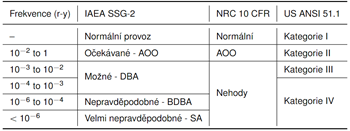
\includegraphics[width=9cm]{img/jad-udalosti.png}
	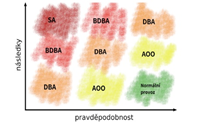
\includegraphics[width=5cm]{img/jad-udalosti1.png}
\end{figure}

\begin{figure}[h!]
    \centering
    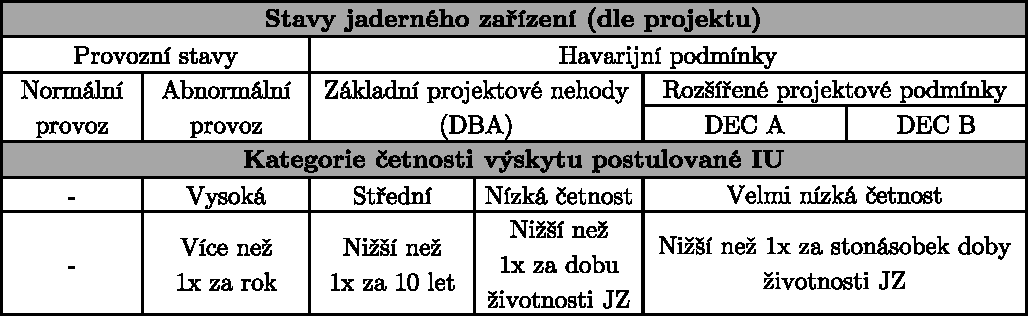
\includegraphics[width=\textwidth]{img/Stavy_JZ_cetnost.pdf}
\end{figure}

\subsubsection{Základní bezpečnostní funkce}

\begin{itemize}
    \item Umožňovat v případě potřeby okamžitě a bezpečně odstavit jaderný reaktor a udržovat jej v podkritickém stavu.
    \item Zabránit nekontrolovanému rozvoji štěpné řetězové reakce
    \item Fyzikálně znemožnit vznik kritického a nadkritického stavu mimo vnitřní prostor jaderného reaktoru.
    \item Zajišťovat odvod tepla vytvářeného jaderným palivem a technologickými systémy.
    \item Zajistit stínění a zabránit úniku radioaktivní látky a šíření ionizujícího záření do životního prostředí.
\end{itemize}

\begin{comment}
    
\subsubsection{Zajištění podkritičnosti}

\begin{itemize}

\item Lze uvažovat všechny existujı́cı́ bezpečnostnı́ systémy (v úrovni
ochrany do hloubky 3a)
\item Při využitı́ každého systému musı́ být uvažována nejvı́ce závažná jednoduchá porucha (navı́c k poruše v rámci metodiky)
\item Na začátku přechodového procesu se obvykle uplatnı́ systém rychlého odstavenı́ reaktoru
\item Následně udrženı́ stabilizovaného podkritického stavu
\end{itemize}
\subsubsection{Zajištění odvodu tepla}

\begin{itemize}
\item Zajištěnı́ technických kritériı́ přijatelnosti pro PIU kategorie AOO nebo DBA
\item Pro PIU AOO přı́snějšı́ kritéria přijatelnosti, za účelem zachovánı́ integrity pokrytı́ palivových elementů (kvůli vyššı́ četnosti výskytu)
\item Nesmı́ dojı́t k nepřijatelnému zvýšenı́ tlaku v I. okruhu nebo II.
okruhu
\item Důsledkem nedostatečného odvodu tepla z AZ může být až eventuelně uvolnění RA látek do I.O. či dále až do ŽP.
\end{itemize}

\subsubsection{Zadržení radioaktivních látek}
\begin{itemize}
\item Neporušenı́ fyzických bariér (s výjimkou bariér porušených
samotnou PIU) se v deterministických analýzách DBE prokazuje
splněnı́m odpovı́dajı́cı́ch radiačnı́ch a technických kritériı́
přijatelnosti
\item Předpokládá, že KNTM je při vzniku PIU a v průběhu jejı́ho
rozvoje hermeticky uzavřen
\item Udrženı́ projektem stanovené těsnosti KTMT musı́ být prokázáno
během rozvoje DBE (i při tlakovému a teplotnı́mu namáhánı́ a
úniku radioaktivnı́ch látek z I.O)
\item KTMT je chráněn proti ztrátě základnı́ bezpečnostnı́ funkce
působenı́m přetlaku systémem řı́zenı́ tlaku a teploty
\end{itemize}


\subsubsection{Zařízení pro jadernou bezpečnost}
\begin{itemize}
    \item zařízení nedůležitá pro JB
    \item zařízení důležitá pro JB = vybraná zařízení - systém nebo komponenta nebo konstrukce důležitá pro jadernou bezpečnost a má vliv na plnění bezpečnostních funkcí, její selhání může vést k ozáření personálu nebo obyvatelstva
    \item zařízení s vlivem na JB které nejsou vybraným zařízením
    \item zařízení pro prevenci rozvoje iniciačních událostí - prostředky pro omezení důsledků selhání vybraných zařízení, prevence rozvoje havarijních podmínek
\end{itemize}

\end{comment}


\textit{Asi by bylo dobré zmínit, že hodnocení jaderné bezpečnosti provádíme buď deterministickými nebo pravděpodobnostními hodnoceními.}

Deterministický přístup:

\begin{itemize}
    \item Definice iniciačních událostí $\rightarrow$ musím aplikovat specifické požadavky.
    \item Určení dostupnosti SKK, okrajových a počátečních podmínek (jednoduchá porucha, zvládání nehody pouze bezpečnostními systémy).
    \item Výběr výpočetního kódu.
    \item Zhodnocení výsledků.
\end{itemize}

Pravděpodobnostní přístup (PSA):

\begin{itemize}
    \item Vychází z deterministických analýz, ale beru v úvahu pravděpodobnost.
    \item Využívám při risk managementu, mám pravděpodobnost, že se něco stane, mohu optimalizovat vůči přínosu.
    \item CDF, pravděpodobnost úniku RA, pravděpodobnost účinku na veřejnost.
\end{itemize}

\subsubsection{Klasifikace událostí}

\begin{itemize}
	\item Fyzikální přístup
	
	\begin{itemize}
		\item Havárie vyvolané kladnou změnou reaktivity (RIA)
		\item Havárie se ztrátou chladiva (LOCA)
		\item Havárie v systému odvodu tepla
		\item Ostatní havárie
		\item Vnější vlivy
	\end{itemize}

	\item Podle iniciačních událostí
	\item stupnice INES
\end{itemize}


\textbf{Havárie vyvolané kladnou změnou reaktivity}

Kladná změna reaktivity v kritickém reaktoru vede ke zvýšení výkonu. Ten závisí na rychlosti a velikosti vložené kladné reaktivity, účinku zpětných vazeb a zásahu regulačního systému. Problém je kritičnost na okamžitých neutronech.

Vliv má na jakém výkonu je reaktor před vložením kladné reaktivity:

\begin{itemize}
    \item Nízký výkon (spouštění) -- nepůsobí zpětné vazby, chování systému je dáno dynamikou nulového reaktoru.
    \item Vysoký (nominální) výkon -- zafungují zpětné vazby, které omezí nárůst výkonu (Doppler), ale parametry reaktoru už jsou blízko limitních hodnot (maximální dovolené teploty) $\rightarrow$ často vede na lokální poškození paliva. Proutek to může vydržet ale tableta se mohla lokálně natavit.
\end{itemize}

Možné  scénáře:

\begin{itemize}
    \item Nekontrolované vysouvání regulačních orgánů = Závisí na maximální rychlosti vysouvání RO a maximální vázané reaktivitě, přechodový proces závisí na výkonu reaktoru (jiné chování u nulového reaktoru a reaktoru na výkonu), nárůst výkonu je omezen zpětnými vazbami a zpravidla nepředstavuje závažné ohrožení.
    \item Vystřelení regulačního orgánu = Teoreticky může nastat při prasknutí pouzdra pohonu RO, v důsledku okamžitého poklesu tlaku v pouzdře dojde k vystřelení tyče z AZ, rychlý proces, ale celková reaktivita je menší než u předchozího, je spojeno s únikem chladiva.
    \item Náhlé uvolnění usazenin absorpčního charakteru (bór) v konstrukci (bór se v průběhu provozu usazuje na konstrukčních částech), při jejich náhlém uvolnění = Kladná změna, rychlý přechodový proces jako vystřelení tyče, závisí na maximální uvolněné reaktivitě.
    \item Nekontrolované snižování koncentrace rozpustných absorbátorů = Chybné snížení koncentrace nebo připojení trasy s čistým kondenzátem, změny koncentrace jsou pomalé $\rightarrow$ prostor pro vyřešení situace nebo odstavení reaktoru, významná změna reaktivity je v řádu hodin.
    \item Chybné zavezení paliva = Dosažení nadkritického stavu z důvodu špatně zavezeného čerstvého PS, vylučuje se zvýšením koncentrace kyseliny borité a administrativní opatření při zavážení PS.
    \item Vtok studené vody do AZ = Uvolnění kladné reaktivity díky zápornému teplotnímu koeficientu reaktivity chladiva (hodnota závisí na koncentraci kyseliny borité).
    \item Vliv tlakových změn = Vliv dutinového koeficientu reaktivity, problém je u vody, která je blízko meze sytosti a v části chladiva probíhá bublinkový var, při záporném dutinovém koeficientu zvýšení tlaku vede ke snížení podílu páry a uvolnění kladné reaktivity.
\end{itemize}

\textbf{Havárie se ztrátou chladiva}

Snížení nebo úplné přerušení chlazení primárního okruhu (SB nebo LB LOCA). Jde o havárie typu LOCA (Loss of Coolant Accident).

Možné  scénáře:

\begin{itemize}
    \item Prasknutí hlavního potrubí IO = LB LOCA, prasknutí potrubí se zachováním plného výtokového průřezu.
    \item Prasknutí potrubí s malým nebo středním únikem = SB LOCA, vyšší pravděpodobnost výskytu a odlišný průběh přechodového procesu, může být horší než u LB LOCA.
    \item Prasknutí trubky v PG = Patří do skupiny progresivních poruch, tj. poruchy, které jsou malé a lokalizované, ale postupně se rozrůstají do vážných rozměrů, šíření poruch ve svazku trubek PG.
\end{itemize}

\textbf{Havárie v systému odvodu tepla}

Jde o poruchy vedoucí ke snížení odvodu tepla z reaktoru. Týkají se primárního i sekundárního okruhu, i odstaveného reaktoru (zbytkový výkon).

Možné  scénáře:

\begin{itemize}
    \item Selhání HCČ = Snížení průtoku vede ke zvýšení teploty a tlaku chladiva v IO $\rightarrow$ ROR, pokud nedojde k ROR otevírá se PV na KO a únik do barbotážního systému, průběh závisí na koncepci IO, počtu vypadlých HCČ, setrvačnosti čerpadel, rychlosti odstavení reaktoru, zásahu obsluhy, ...
    \item Nestability proudění chladiva v AZ = Snížení průtoku v některých kanálech AZ nebo skupině kanálů vede k narušení hydrodynamiky AZ a přehřátí části PP, příčinou havárie může být částečné zablokování průtoku chladiva CP (cizí předmět) nebo vznik varu v některém PS (vyšší hydraulický odpor).
    \item Selhání dodávky napájecí vody do PG = hodně možností, tj. vyšší relativní četnost poruchy (hlavní příčiny - selhání napájecích čerpadel, výpadek napětí v síti vlastní spotřeby, prasknutí potrubí napájecí vody), havarijní analýzy řeší následek prasknutí hlavního napájecího kolektoru s oboustranným výtokem (Loss of Feedwatter - LOFW) $\rightarrow$ uzavření ventilu na napájecí trase kvůli zamezení výtoku vody z PG, v PG roste tlak, snižuje se hladina na sekundární straně, v IO roste teplota a tlak.
    \item Prasknutí HPK nebo hlavního parovodu = Nejhorší havárie na parním potrubí IIO, důsledkem je prudký pokles tlaku a teploty na teplotu sytosti v IIO, pokles tlaku v IIO vyvolá signál pro zvýšení výkonu reaktoru a zvýšení dodávek napájecí vody do PG, to vede k snížení teploty, objemu a tlaku v IO a dalšímu zvýšení výkonu díky zpětným vazbám.
    \item Selhání hlavních systémů odvodu tepla v kondenzátoru = Poruchy chlazení kondenzátorů TG vedou k odstavení TG.
\end{itemize}

\textbf{Ostatní havárie}

Zahrnuje situace, které mohou nastat při odstávkách nebo v systémech, které přímo nesouvisí s provozem reaktoru. Tyto události mohou vést k rozsáhlému úniku RA látek.

Možné scénáře:

\begin{itemize}
    \item Havárie při manipulaci s palivem = Čerstvé (havárie s kritičností) nebo ozářené palivo (kritičnost a ztráta chlazení v bazénu VJP).
    \item Havárie systému zpracování RAO = Události při skladování, přepracování a ukládání RAO.
\end{itemize}

\textbf{Vnější vlivy}

\begin{itemize}
    \item Velmi málo pravděpodobné povětrnostní podmínky a živelní pohromy.
    \item Vlivy vyplývající z lidské činnosti.
    \item Zemětřesení.
    \item Záplavy, průtrž mračen, vítr.
    \item Požáry.
    \item Tlaková vlna (důsledek výbuchu).
    \item Pád letadla.
    \item Sabotáže.
\end{itemize}

\subsection{Nehody}

\subsubsection{Projektové nehody (DBA)}

DBA přestavují základní sadu událostí, které musí být pokryty bezpečnostními systémy, tak aby nedošloze k překročení odpovídajících referenčních úrovní nebo limitů ozáření.

\begin{itemize}
    \item Zvládnutí DBA je nezbytné pro vyhodnocení přijatelnosti návrhu reaktoru.
    \item Při DBA je jedna nebo více bezpečnostních funkcí je napadena.
    \item Pro zvládnutí události je nutný zásah bezpečnostních systémů.
    \item DBA by neměly mít dopad na okolí elektrárny a veřejnost.
    \item Zpravidla se během provozu elektrárny nevyskytne.
    \item Frekvence výskytu $10^{-4}$ až $10^{-2}$ za 1 rok.
\end{itemize}

\textbf{Hodnocení bezpečnosti:}

\begin{itemize}
    \item Proces komplexního deterministického hodnocení a PSA.
    \item Hodnocení prokazuje, že JZ plní v rozsahu projektových východisek požadavky na JB a RO při normálním a abnormálním provozu.
    \item Plnění bezpečnostních funkcí je v analýzách zajišťováno jen bezpečnostními systémy.
    \item Musí být zahrnuto kritérium jednoduché poruchy (uvažuje se nejzávažnější možná porucha).
    \item Dopad PIE na bezpečnostní systémy je konzervativně volen jako nejhorší $\rightarrow$ nejméně příznivý průběh události.
    \item Zohledňují se nejistoty a výrobní tolerance.
    \item Deterministické hodnocení -- pro všechny PIE $\rightarrow$ následky nehody.
    \item Pravděpodobnostní hodnocení $\rightarrow$ pravděpodobnost CDF a LRF.
\end{itemize}

\subsubsection{Nadprojektové nehody (BDBA)}

Jde o PIE vedoucí k DBA spolu s dalším selháním bezpečnostních systémů $\rightarrow$ vyvolané scénáři závažnějšími než základní projektová nehoda. Např. ztráta ECCS během LOCA, ATWS (událost spojená s neodstavením reaktoru při vyžádání jeho odstavení, např. selhání pádu tyče), totální ztráta napájecí vody, SBO.

\begin{itemize}
    \item V odezvě na BDBA se zpravidla objevují akce operátorů na zmírnění důsledků nehody:
    \begin{itemize}
        \item Odpouštění a doplňování chladiva v IO (snižování tlaku přes KO, doplňování vody přes ECCS).
        \item Odpouštění a doplňování chladiva v IIO (PV, havarijní napájení PG).
        \item Hermetizace (izolace) KNTM.
        \item Odtlakování KNTM (ventilace KNTM).
    \end{itemize}
\end{itemize}

\textbf{Hodnocení bezpečnosti:}

\begin{itemize}
    \item Na základě deterministického a pravděpodobnostního hodnocení vybrány bezpečnostně nejvýznamnější BDBA události.
    \item Jedná se o PIE vedoucí k DBA + rozšířené podmínky, např. nedostupnost ECCS během LOCA, SBO.
    \item Velmi málo pravděpodobné události.
    \item V bezpečnostních analýzách se používají méně konzervativní kritéria.
    \item Mohou být použity realistické předpoklady $\rightarrow$ best-estimate přístup -- neuvažuje se kritérium jednoduché poruchy, počítá se se zásahem systémů, které nejsou bezpečnostní.
    \item Hodnotí se průběhy i radiační následky (identifikace nutných opatření, podklady pro návody zvládání RMU a výcvik obsluhy, ...)
\end{itemize}

\subsubsection{Těžké havárie (SA)}

Důsledkem je poškození AZ, roztavení paliva a případně i významný únik RA látek.

\begin{itemize}
    \item Procesy v RN: poškození paliva (oxidace Zr při vysokých teplotách, 1200 $^\circ$C), parní exploze, porušení integrity.
    \item Poškození RN.
    \item Procesy mimo RN: zahřívání povrchů, exploze vodíku, interakce betonu s kóriem.
\end{itemize}

\subsection{Mezinárodní stupnice -- INES}

= The International Nuclear Event Scale

\begin{itemize}
    \item Vyvinuta v roce 1990 (IAEA).
    \item Určena pro rychlou orientaci veřejnosti. Je to komunikační nástroj, který usnadňuje komunikaci mezi odbornou a laickou veřejností a médii.
    \item Používá se pro hodnocení událostí na všech zařízeních souvisejících s jaderným průmyslem.
    \item Dodatečně rozšířena pro potřeby událostí spojených s dopravou, skladováním a použitím radioaktivních látek a zdrojů záření.
    \item Zahrnuje ztrátu nebo krádež RA zářičů, nález opuštěných zářičů či neplánované ozáření osob při regulovaných dozorovaných činnostech.
    \item Neslouží pro srovnávání bezpečnosti jednotlivých elektráren.
    \item Neslouží pro hodnocení zabezpečení zdrojů IZ.
    \item Nevztahuje se na události spojené pouze s technickou bezpečností a pro události, které nemají vztah k jaderné nebo radiační bezpečnosti, tj. únik chemikálií, zásah elektrickým proudem, události ovlivňující pohotovost turbíny nebo generátoru, pokud nebyl ovlivněn výkon reaktoru. Jedná se tedy spíše o radiologickou než technologickou stupnici.
\end{itemize}

\textbf{Klasifikace do sedmi stupňů:}

\begin{itemize}
	\item Stupeň 4-7 -- havárie (accidents).
	\item Stupeň 1-3 -- nehody (incidents).
	\item Stupeň 0/pod stupnicí -- události bez vlivu na bezpečnost.
\end{itemize}
	
Bezpečnostní význam mají události 2. a vyššího stupně. Většina hlášených událostí je do 3. stupně.

\begin{figure}[h!]
	\centering
	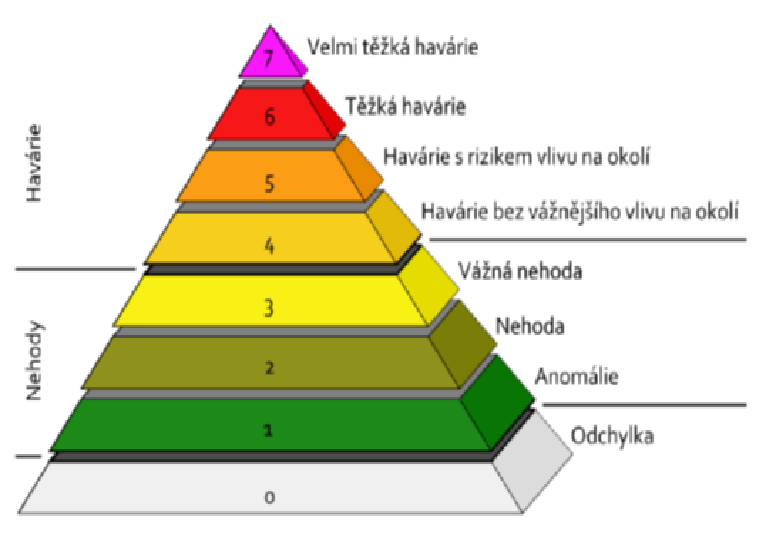
\includegraphics[width=8cm]{img/ines.png}
	\caption{INES}
	\label{fig:ines} 
\end{figure}

\begin{itemize}
	\item[0)] \textbf{Událost bez vlivu na bezpečnost}.
	\item[1)] \textbf{Anomálie} = technická porucha nebo odchylka od schváleného režimu, ale se zbývající významnou hloubkovou ochranou.
	\item[2)] \textbf{Nehoda} = nehoda s významným selháním bezpečnostních opatření, ale se zbývající dostatečnou hloubkovou ochranou k vypořádání se dodatečnými poruchami.
	\item[3)] \textbf{Vážná nehoda} = významné vnitřn.í poškození ovšem bez nutnosti vnějšího zásahu, další porucha bezpečnostních systémů by mohla vést k havarijním podmínkám.
	\item[4)] \textbf{Havárie bez vážnějšího rizika} = havárie vně zařízení, bez významného vlivu na okolí, významné poškození zařízení (např. částečné tavení AZ), ozáření jednotlivců z obyvatelstva na úrovni ročních limitů pro obyvatelstvo, ozáření pracovníků na úrovni možných časných úmrtí.
	\item[5)] \textbf{Havárie s rizikem} = havárie vně zařízení, těžké poškození jaderného zařízení (havárie s kritičností, velký požár a exploze), únik významného množství radioaktivity, aplikace opatření pro snížení rizika poškození zdraví u obyvatelstva.
	\item[6)] \textbf{Těžká havárie} = velký únik radioaktivity do životního prostředí, plná aktivace opatření pro snížení pravděpodobnosti zdravotních následků u obyvatelstva.
	\item[7)] \textbf{Velmi těžká havárie} = únik velmi velkého množství radioaktivity, možnost akutních zdravotních účinků, dlouhodobé poškození životního prostředí, vliv přesahuje hranice států.
\end{itemize}

\textbf{Kritéria hodnocení dle INES:}

Každá událost se hodnotí vzhledem ke třem kritériím, přičemž výsledné hodnocení je dáno nejvyšším stupněm dle všech tří kritérií.

\begin{itemize}
    \item Obyvatelé a ŽP (stupně 2-7):
    Je založeno na dávkách obyvatel, tj. obdržená dávka a počet ozářených osob. Vzhledem k použití havarijních opatření můžou být obdržené dávky velmi nízké
    \item Radiační bariéry a opatření (stupně 2-5):
    Je založeno na množství uvolněných radioaktivních látek. Pro zahrnutí širokého spektra radioaktivních izotopů, které se mohou uvolnit do ŽP se používá koncept radiačního ekvivalentu $^{131}$I. Jsou definovány konverzní faktory pro jednotlivé izotopy.
    \item DID (stupně 1-3).
\end{itemize}

INES poskytuje rychlou zprávu o významu události $\rightarrow$ klasifikace na základě prvotního odhadu, avšak hodnocení se může měnit podle vývoje situace. Výsledné hodnocení je dáno nejvyšším stupněm podle všech tří kritérií! Ve výsledku se bere nejvyšší stupeň, a to z důvodu, že u jednoho kritéria může být výsledkem stupeň 1, ale z pohledu jiného může být mnohem výše.

\textbf{Dávky pro jednotlivce:}

Kritérium obdržené dávky je nejpřímější kritériem. Definice se vztahují k dávkám, které byly obdrženy, nebo velmi pravděpodobně mohly být obdrženy (tj. zvážit výskyt obdržených dávek, o kterých se nevědělo). Hodnocení vychází z ozáření jedné osoby, ozáření více osob je důvodem ke zvýšení hodnocení až o dva stupně.

\begin{itemize}
    \item Stupeň 4: výskyt smrtelného deterministického účinku. 
    Pravděpodobný výskyt smrtelného deterministického účinku v důsledku celotělového ozáření (absorbovaná dávka řádu několika Gy).
    \item Stupeň 3: výskyt nebo pravděpodobný výskyt deterministických účinků, při nichž nedojde ke smrti.
    Ozáření vedoucí k efektivní dávce vyšší než je 10x stanoveného ročního limitu pro pracovníky se zářením 20 mSv.
    \item Stupeň 2: ozáření jednoho obyvatele vedoucí k efektivní dávce přesahující 10 mSv.
    Ozáření pracovníka přesahující stanovené roční limity.
    \item Stupeň 1: ozáření jednoho obyvatele přesahující roční dávkové limity.
    Kumulativní ozáření pracovníka nebo obyvatele přesahující stanovené roční limity.
\end{itemize}

\subsubsection{Příklady událostí}

\begin{itemize}
	\item[1)] Porušení technických podmínek, nehody bez přímých důsledků, které odhalí nedostatky v organizačním systému nebo kultuře bezpečnosti, menší defekty v potrubí.
	\item[2)] Ishikava (Japonsko), Mihama (Japonsko, 1991), Atucha (Argentina), Forsmark (švédsko), Cadarache (Francie), Pickering A-B (Kanada, 2003)
	\item[3)] Selafield (UK), Paks (Maïarsko, 2002)), Vandellos (španělsko, 1989), Davis Besse-1, (USA, 2002)
	\item[4)] Jaslovské Bohunice (Slovenská rep.), Windscale Pile (VB, 1973), Saint Laurent (Francie, 1980), Tokaimura (Japonsko, 1999)
	\item[5)] TMI2 (USA, 1979), Chalk River (Kanada), Windscale Pile (VB, 1957)
	\item[6)] Kyštym (Majak) (Rusko, 1957) -- obohacovací závod
	\item[7)] Chernobyl (Ukrajina, 1986), Fukushima (Japonsko, 2011)
\end{itemize}

\begin{figure}[h!]
    \centering
    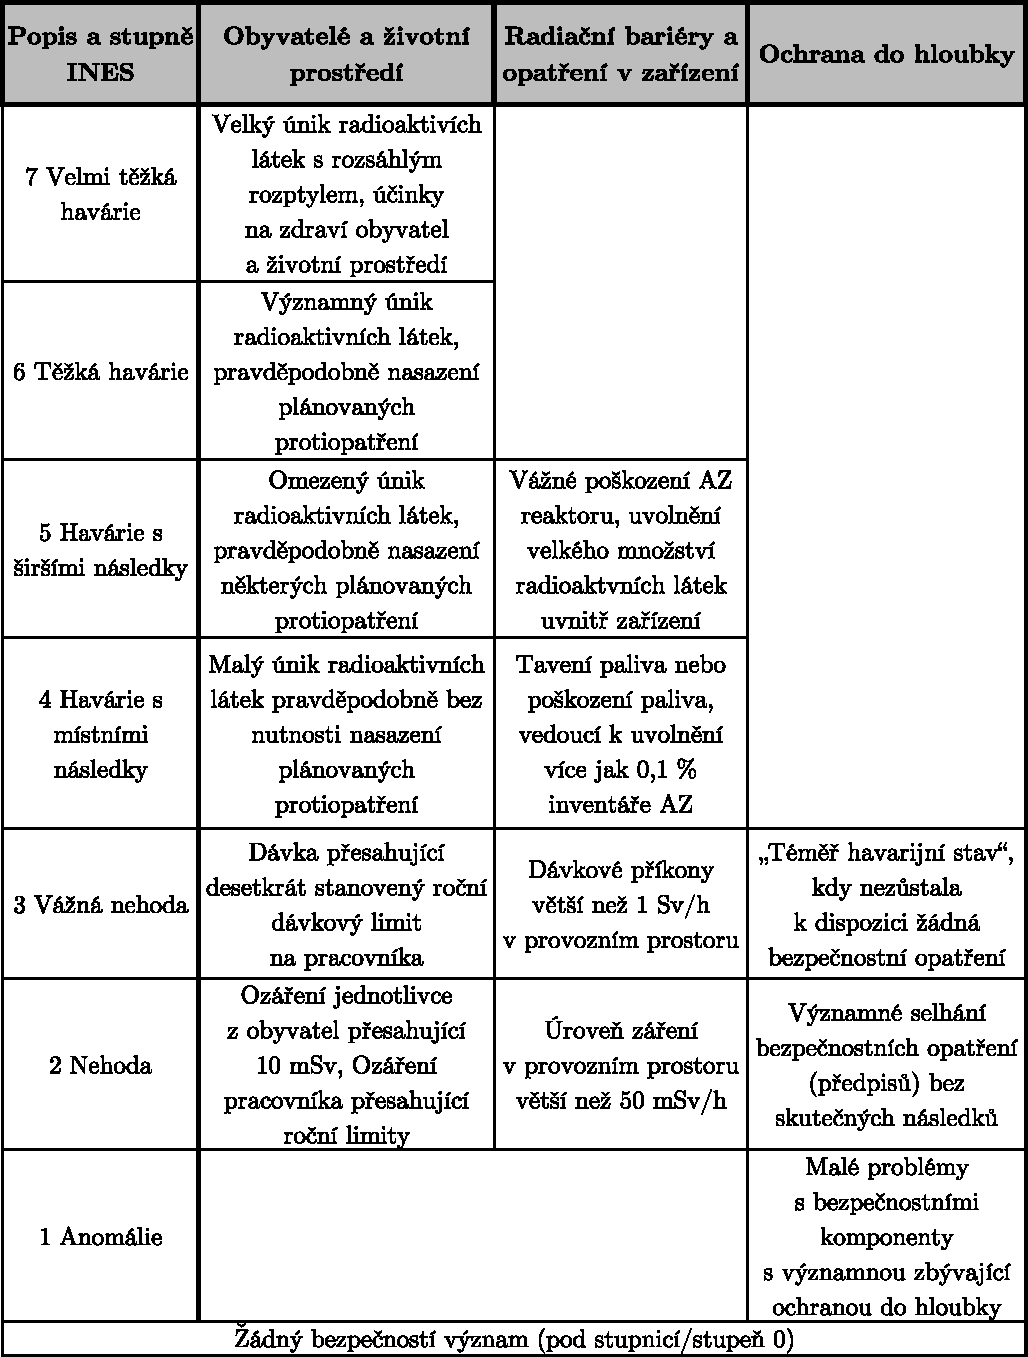
\includegraphics[width=0.9\textwidth]{img/INES_tab.pdf}
\end{figure}